\section{XML基本语法}

\begin{frame}{CH2 XML基本语法}
\begin{figure}
    
\includegraphics[width=0.9\textwidth]{figure/cover.png}
\end{figure}
\end{frame}

\begin{frame}{本章学习目标}
\begin{itemize}
\item 掌握XML的文档组成结构
\item 掌握XML声明、处理指令、注释、元素、属性、命名空间等基本概念
\item 能够编写格式良好的XML文档
\end{itemize}
\end{frame}

\begin{frame}[fragile]{目录}
\begin{easylist} \easyitem
& XML文档结构
& 元素
&& 元素和标记
&& 元素的内容
&& 元素的嵌套
& 属性
&& 属性的语法形式
&& 属性的使用场景
&& 属性的命名规范
&& 属性值
& 命名空间
& XML文档规范级别
\end{easylist}
\end{frame}

\subsection{2.1 XML文档结构}

\begin{frame}{2.1 XML文档结构}
\par XML本身侧重于数据的表示,并通过CSS、XSLT等技术把数据以指定的格式进行呈现,实现数据表示与呈现的分离。
\end{frame}


\begin{frame}[fragile, allowframebreaks]{示例XML文档}
\begin{lstlisting}[tabsize=8, basicstyle=\small\tt, language=XML]
<?xml version="1.0" encoding="UTF-8" standalone="yes"?>
<?xml-stylesheet type="text/css" href="2-1.css"?>
<!-- 个人通讯录 -->
<addressList>
    <group name="同学">
        <person>
            <name>吴泽林</name>
            <birthday>1985-09-11</birthday>
            <mobile>135-1234-5678</mobile>
            <telephone>68689999</telephone>
            <email>wuzelin@163.com</email>
            <address>漳州</address>
        </person>
    </group>
    <group name="网友">
        <person>
            <name>罗中华</name>
            <mobile>136-1111-1118</mobile>
            <telephone>22339999</telephone>
            <email>luozh@163.com</email>
            <address>北京</address>
        </person>
    </group>
</addressList>

<!-- 处于篇幅考虑,书中源代码内容有删减,读者可以通过附带源码
查看更多信息 -->
\end{lstlisting}
\end{frame}


\begin{frame}{文档构成}
\par 一个XML文档由序言、主体和尾声三部分构成
\begin{itemize}
\item 序言(Prolog): 从XML声明到文档根元素开始前的部分,包括XML声明、注释和处理指令等,序言是可选的
\item 文档主体(Body): 文档根元素及其所包含的内容,每一个XML文档有且仅有一个根元素
\item 尾声(Epilog): 文档根元素后面的部分,可以包含注释、处理指令以及空白信息,一般不出现
\item 一个XML文档最基本的语法要素包括:XML声明、处理指令、注释和XML元素.
\end{itemize}
\end{frame}


\begin{frame}{文档声明}
\begin{shaded}
<?xml version="1.0" encoding="UTF-8" standalone="yes"?>
\end{shaded}

\begin{itemize}
\item version
\item  encoding
\item standalone
\end{itemize}
\end{frame}


\begin{frame}{处理指令}
\begin{shaded}
\par 语法形式: <?处理指令名称 处理指令信息?>
\par E.g. <?topdf path="/pdf-files" ?>
\end{shaded}

\begin{itemize}
\item 处理指令PI(Processing Instruction)是XML文档中为XML处理程序提供必要的处理信息的指令描述。XML解析器会把它原封不动地传递给XML应用程序,由应用程序来根据该指令进行必要处理,或者再把它原封不动地传递给下一个应用程序。
\item  处理指令如何解释完全由外部应用程序决定
\item xml-stylesheet问题
\end{itemize}
\end{frame}


\begin{frame}{注释}
\begin{shaded}
\par 语法形式: <!-- 注释正文 -->
\end{shaded}

\begin{itemize}
\item 注释本身不能放入到标记之内
\item  注释正文中不能出现连续的“--”符号
\item 注释不能以“--->”符号串结尾,也不能放到XML文档声明之前
\item 可以对标记进行注释
\item 注释不能嵌套使用
\end{itemize}
\end{frame}


\begin{frame}[fragile]{注释本身不能放入到标记之内}
\begin{lstlisting}[tabsize=8, basicstyle=\small\tt, language=XML]
<?xml version="1.0" encoding="UTF-8"?>
<document>
    <head <!--This is the heading element-->>
        注释测试例子
    </head>
    <body>正文内容</body>
    </message>
</document>
\end{lstlisting}
\end{frame}


\begin{frame}[fragile]{注释正文中不能出现连续的“--”符号}
\begin{lstlisting}[tabsize=8, basicstyle=\small\tt, language=XML]
<?xml version="1.0" encoding="UTF-8"?>
<document>
    <head>注释测试例子</head>
    <!--这是正文内容--夏天-->
    <body>正文内容</body>
    </message>
</document>
\end{lstlisting}
\end{frame}


\begin{frame}[fragile]{注释不能以“--->”结尾,不能放到文档声明之前}
\begin{lstlisting}[tabsize=8, basicstyle=\small\tt, language=XML]
<!-- 该注释后面是XML声明 -->
<?xml version="1.0" encoding="UTF-8"?>
<document>
    <head>注释测试例子</head>
    <!--这是正文内容-夏天--->
    <body>正文内容</body>
    </message>
</document>
\end{lstlisting}
\end{frame}


\begin{frame}[fragile]{可以对标记进行注释}
\begin{lstlisting}[tabsize=8, basicstyle=\small\tt, language=XML]
<?xml version="1.0" encoding="UTF-8"?>
<document>
    <!--
    <head>注释测试例子</head>
    <body>正文内容</body>
    </message>
    -->
</document>
\end{lstlisting}
\end{frame}


\begin{frame}[fragile]{注释不能嵌套使用}
\begin{lstlisting}[tabsize=8, basicstyle=\small\tt, language=XML]
<?xml version="1.0" encoding="UTF-8"?>
<document>
    <!--
    <head>注释测试例子</head>
    <!-- 这是正文内容-夏天 -->
    <body>正文内容</body>
    </message>
    -->
</document>
\end{lstlisting}
\end{frame}



\subsection{2.2 元素}

\begin{frame}{2.2 元素}
\par 元素(Element)是XML文档的基本构成单元,它表示了文档的结构和文档中包含的数据,格式良好的XML文档必须拥有一个唯一的根元素。
\begin{itemize}
\item 元素和标记
\item  元素内容
\item 元素的嵌套
\end{itemize}
\end{frame}

\subsubsection{2.2.1 元素和标记}
\begin{frame}{元素和标记}
\begin{shaded}
\par 元素的基本语法形式: <标记>元素内容</标记>
\par 标记的基本语法形式:<标记名 [[属性名1="属性值1"] [属性名2="属性值2"] …]>
\end{shaded}
\begin{itemize}
    \item 标记区分大小写
    \item  标记必须配对出现
    \item 标记首字符以字母、下划线“\_”、冒号“:”以及Unicode字符集中的某一部分开始,支持汉字; 其他部分可以是字母、数字、下划线“\_”、连字符“-”、句点“.”、冒号“:”,以及Unicode字符集中的某一部分
    \item 标记不能包含空格符号或斜线符号“/”
\end{itemize}
\end{frame}


\begin{frame}{标记示例}
\begin{itemize}
    \item 有效的非空标记示例:<address>漳州</address>
    \item 有效的空标记示例:  <img src="test.jpg"/>
    \item 无效标记示例:      <address>漳州</Address>
    \item 无效标记示例:      <p>段落内容之一<p>段落内容之二
\end{itemize}
\end{frame}


\subsubsection{2.2.2  元素的内容}
\begin{frame}{2.2.2  元素的内容}
\par 元素内容可以包括被解析字符数据(Parsed Character Data)、字符数据CDATA段、以及处理指令和注释
\end{frame}


\begin{frame}{被解析字符数据}
\par 被解析字符数据部分可以是任意合法的Unicode字符,但是不能包含被用作特殊用途的字符,例如标记的开始符号“<”。
\par 通过实体转义的方式解决特殊字符问题
\begin{center}
    \begin{tabular}{|c|c|}
    \Xhline{1.3pt}
    字符 &    引用方式 \\
    \Xhline{1.3pt}
     < & \&lt;  \\
     \hline
     > & \&gt;  \\
    \hline
    \& & \&amp;  \\
    \hline
    ' & \&quot;  \\
    \hline
    " & \&apos;  \\
    \hline
    \end{tabular}
\end{center}
\end{frame}


\begin{frame}[fragile]{给书名加上书名号}
\begin{lstlisting}[tabsize=8, basicstyle=\small\tt, language=XML]
<?xml version="1.0" encoding="UTF-8"?>
<books>
    <book>
        <title>XML原理与应用</title>
        <authro>夏天</authro>    
    </book>
</books>
\end{lstlisting}
\end{frame}


\begin{frame}{CDATA段}
\begin{shaded} 
\par 基本语法形式: <![CDATA[ 文本内容 ]]>
\par 有利于处理包含大量特殊符号的文本当作普通文本处理的情况
\end{shaded}
\end{frame}

\begin{frame}[fragile]{采用实体转义方式}
\begin{lstlisting}[tabsize=8, basicstyle=\small\tt, language=XML]
<?xml version="1.0" encoding="UTF-8"?>
<demo>
    <content>
        &lt;group name="同学"&gt;
            &lt;person&gt;
                &lt;name&gt;吴泽林&lt;/name&gt;
                &lt;birthday&gt;1985-09-11&lt;/birthday&gt;
                &lt;mobile&gt;135-1234-5678&lt;/mobile&gt;
                &lt;telephone&gt;68689999&lt;/telephone&gt;
                &lt;email&gt;wuzelin@163.com&lt;/email&gt;
                &lt;address&gt;漳州&lt;/address&gt;
            &lt;/person&gt;
        &lt;/group&gt;
    </content>
</demo>
\end{lstlisting}
\end{frame}

\begin{frame}[fragile]{采用CDATA方式}
\begin{lstlisting}[tabsize=8, basicstyle=\small\tt, language=XML]
<?xml version="1.0" encoding="UTF-8"?>
<demo>
    <content>
        <![CDATA[
        <group name="同学">
            <person>
                <name>吴泽林</name>
                <birthday>1985-09-11</birthday>
                <mobile>135-1234-5678</mobile>
                <telephone>68689999</telephone>
                <email>wuzelin@163.com</email>
                <address>漳州</address>
            </person>        
        </group>
        ]]>
    </content>
</demo>
\end{lstlisting}
\end{frame}




\subsubsection{2.2.3 元素的嵌套}
\begin{frame}[fragile]{2.2.3 元素的嵌套}
\begin{easylist} \easyitem
& 元素描述了XML文档的逻辑结构,对于一个复杂的文档来说,单纯用一组并列的元素是无法准确刻画其结构关系的,通过在元素中嵌套子元素可以更好地描述XML文档数据之间的语义关联性。同时,也可以根据元素之间的嵌套关系把整个XML文档看成是一棵具有严格层次关系的树,方便数据的查询、定位和处理。
& XML的元素之间虽然可以嵌套使用,但不能交叉重叠嵌套,例如以下写法是错误的:
& <h1>中国<b>古代文明</h1></b>
\end{easylist}
\end{frame}



\subsection{2.3 属性}

\begin{frame}[fragile]{2.3 属性}
\par 属性是元素的可选组成部分,用于对元素及其内容的附加信息进行说明
\begin{easylist} \easyitem
& 属性的语法形式
& 属性的使用场景
& 属性的命名规则
& 属性值
\end{easylist}
\end{frame}

\subsubsection{2.3.1 属性的语法形式}
\begin{frame}[fragile]{属性的语法形式}
\begin{easylist} \easyitem
& 非空元素如下:
&& <标记名 属性名1="属性值1" 属性名2="属性值2" …] >元素内容</标记名>
&& <标记名 属性名1='属性值1' 属性名2='属性值2' …] />元素内容</标记名>
& 空元素如下:
&& <标记名 属性名1="属性值1" 属性名2="属性值2" … />
&& <标记名 属性名1='属性值1' 属性名2='属性值2' … />
& E.g. <person group="同学"></person>
\end{easylist}

\end{frame}


\subsubsection{2.3.2 属性的使用场景}
\begin{frame}[fragile]{属性的使用场景}
\begin{easylist} \easyitem
& 属性的使用
&& 与XML文档阅读者无关的简单信息建议使用属性
&& 与XML文档有关但是与XML文档的内容无关的简单信息建议使用属性
&& 元素与属性的具体使用有争论,需要灵活掌握
& 属性的不足
&& 属性不能包含多个值(元素可以)
&& 属性不容易被扩充(方便将来的修改)
&& 属性不能描述结构(子元素可以)
&& 属性更难被程序代码处理
&& 属性值不容易进行DTD测试
\end{easylist}
\end{frame}


\subsubsection{2.3.3 属性的命名规则}
\begin{frame}[fragile]{属性的命名规则}
\begin{easylist}
& 属性的命名规则和元素相似
& 同一个元素内不能包含多个同名属性,例如以下反例:\\ <todo date="2050-05-05" date="2150-05-05" />
\end{easylist}
\end{frame}


\subsubsection{2.3.4 属性值}
\begin{frame}[fragile]{属性值}
\begin{easylist}
& 属性值必须用单引号或双引号括起来,不能混用
& 双引号括起来的属性值中可以出现单引号,反之亦然
& 属性值不能直接包括“<”符号,但可以包含''>''
& 属性值不能直接包括“\&”符号,除非引用实体
\end{easylist}
\end{frame}

\begin{frame}[fragile]{非法属性值示例}
\begin{easylist}
& <todo status="important("special")"/>  \\ <!-- 用双引号括起来的字符串中不能直接包含双引号 -->
& <todo status="important > urgent"/>   \\ <!--  属性值中不能直接包含小于号 -->
& <todo status="important \& urgent"/>  \\ <!-- 属性值中不能直接包含“\&” -->
& <todo status="important'/>  \\ <!-- 属性值不能用一个单引号和一个双引号括起来 -->
& <todo status=important/>   \\ <!-- 属性值必须用引号括起来 -->
\end{easylist}
\end{frame}


\subsection{2.4 命名空间}

\begin{frame}[fragile]{命名空间问题}
\par 人力资源维护的员工信息:
\begin{lstlisting}[tabsize=8, basicstyle=\small\tt, language=XML]
<?xml version="1.0"?>
<employees>
    <employee>
        <name>金成</name>
        <birthday>1982-08</birthday>
        <hiredate>2005-09</hiredate>
        <major>软件开发</major>
        <projects>
            <project name="项目A" role="工程师" year="2006"/>
            <project name="项目B" role="架构师" year="2007"/>
        </projects>
    </employee>
</employees>
\end{lstlisting}
\end{frame}


\begin{frame}[fragile]{命名空间问题}
\par 你认为该员工表现优秀,应该增加薪水以示奖励,此时,可在XML文件中增加一条评论:“表现优秀,增加10\%薪水”
\begin{lstlisting}[tabsize=8, basicstyle=\small\tt, language=XML]
<?xml version="1.0"?>
<employees>
    <employee>
        <name>金成</name>
        <birthday>1982-08</birthday>
        <hiredate>2005-09</hiredate>
        <major>软件开发</major>
        <comment>表现优秀,增加10%薪水</comment>
        <projects>
            <project name="项目A" role="工程师" year="2006"/>
            <project name="项目B" role="架构师" year="2007"/>
        </projects>
    </employee>
</employees>
\end{lstlisting}
\end{frame}


\begin{frame}[fragile]{命名空间问题}
\par 人力资源管理人员根据老板的评论,加入了自己的注释
\begin{lstlisting}[tabsize=8, basicstyle=\small\tt, language=XML]
<?xml version="1.0"?>
<employees>
    <employee>
        <name>金成</name>
        <birthday>1982-08</birthday>
        <hiredate>2005-09</hiredate>
        <major>软件开发</major>
        <comment>表现优秀,增加10%薪水</comment>
        <comment>薪水已调整</comment>
        <projects>
            <project name="项目A" role="工程师" year="2006"/>
            <project name="项目B" role="架构师" year="2007"/>
        </projects>
    </employee>
</employees>
\end{lstlisting}
\end{frame}

\begin{frame}[fragile]{问题}
\par 由于老板和人力资源管理人员都可能向原XML文件中增加同样的标记<comment>,日后再来阅读该文件时,便极有可能增加语义混淆:
\begin{easylist}
& 哪一些评论是老板增加的?
& 哪一些是人力部门工作人员增加的?
\end{easylist}
\end{frame}


\begin{frame}[fragile, allowframebreaks]{使用命名空间}
\begin{shaded}
\par 语法形式: xmlns:命名空间前缀="命名空间名"
\end{shaded}
\begin{lstlisting}[tabsize=8, basicstyle=\small\tt, language=XML]
<?xml version="1.0"?>
<hr:employees xmlns:hr="http://www.demo.org/human_resources"
    xmlns:boss="http://www.demo.org/big_boss">
    <hr:employee>
        <hr:name>金成</hr:name>
        <hr:birthday>1982-08</hr:birthday>
        <hr:hiredate>2005-09</hr:hiredate>
        <hr:major>软件开发</hr:major>
        <boss:comment>表现优秀,增加10%薪水</boss:comment>
        <hr:comment>薪水已调整</hr:comment>
        <hr:projects>
            <hr:project name="项目A" role="工程师" year="2006"/>
            <hr:project name="项目B" role="架构师" year="2007"/>
        </hr:projects>
    </hr:employee>
</hr:employees>
\end{lstlisting}
\end{frame}

\begin{frame}{使用命名空间}
\par 根据教材进一步了解默认命名空间和命名空间的作用域
\end{frame}


\subsection{2.5 XML文档的规范级别}

\begin{frame}[fragile]{2.5 XML文档的规范级别}
\begin{easylist} \easyitem
& 格式良好的XML文档
&& 符合XML语法要求
& 有效的XML文档
&& 格式良好,满足约束条件
& 规范化的XML文档
&& 判定两个XML文件在信息集合的角度看是否一致的方法
\end{easylist}
\end{frame}


\begin{frame}
\begin{center}
    \Huge END
\end{center}
\begin{figure}
    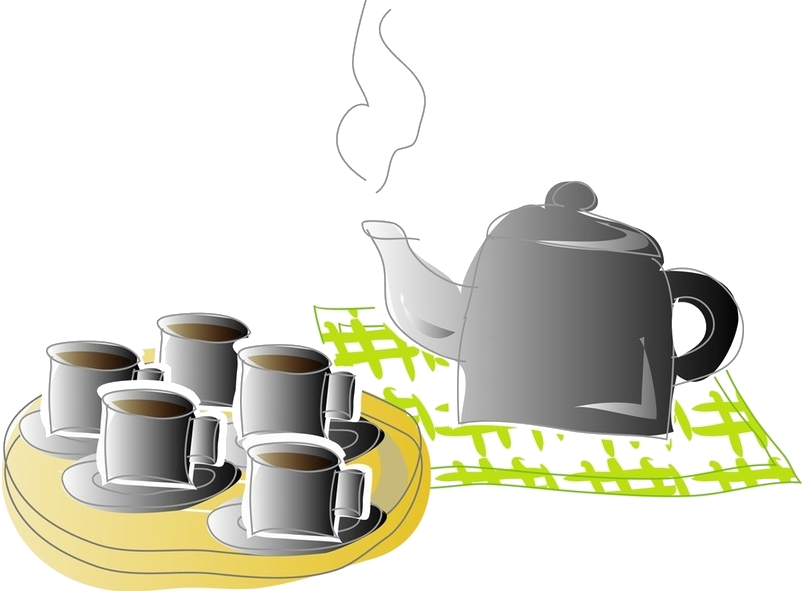
\includegraphics[width=0.75\textwidth]{figure/relax.png}
\end{figure}
\end{frame}